\documentclass[useAMS,usenatbib]{mn2e}

\usepackage{graphicx}
\usepackage{float}
\usepackage{amsmath}
\usepackage{amssymb}
\usepackage{cite}
\usepackage{natbib}
\usepackage{xcolor}

\def\aap{Astronomy \& Astrophysics}
\def\apj{The Astrophysical Journal}
\def\mnras{Monthly Notices of the Royal Astronomical Society}

\usepackage{newtxtext,newtxmath}
\usepackage[T1]{fontenc}
\usepackage{ae,aecompl}
\usepackage{hyperref}

\newcommand{\red}[1]{{\color{red} #1}}

%%%%%%%%%%%%%%%%%%% TITLE PAGE %%%%%%%%%%%%%%%%%%%


\title[SL Challenge]{The Strong Gravitational  Lens Finding Challenge}

\author[R. B. Metcalf {\it et al.}]{
R. Benton Metcalf,$^{1,4}$\thanks{E-mail: robertbenton.metcalf@unibo.it} M. Meneghetti,$^4$ R\'emi Cabanac,$^2$ Emmanuel Bertin,$^3$ Alessandro Sonnenfeld,$^5$ and \\
% List of institutions
$^{1}$ Departimento di Fisica \& Astronomia, Universit\`a di Bologna, viale Berti Pichat 6/2, 40127 Bologna, Italy \\
$^{2}$ IRAP, University of Toulouse, CNRS, UPS, France.\\
$^{3}$ Sorbonne Universités, UPMC Univ. Paris 6 and CNRS, UMR 7095, Institut d'Astrophysique de Paris,  98bis Bd Arago, F-75014, Paris \\
$^{4}$ INAF-Osservatorio Astronomico di Bologna, via Ranzani 1, 40127 Bologna, Italy \\
$^{5}$Kavli IPMU (WPI), UTIAS, The University of Tokyo, Kashiwa, Chiba 277-8583, Japan\\
}

\begin{document}

\date{Accepted . Received ; in original form }

\maketitle

\label{firstpage}

% Abstract of the paper
\begin{abstract}

\end{abstract}

\begin{keywords}
gravitational lensing -- cosmology 
\end{keywords}


\section{Introduction}

some numbers about future surveys

\section{The Challenge}

\section{the simulations}

\section{lens finding methods}

This section contains short descriptions of the lens finding methods that were used in 
the challenge.  Each subsection refers to a team which gave a separate entry.

\subsection{GAHEC IRAP (Remi Cabanac)}

\begin{figure}
 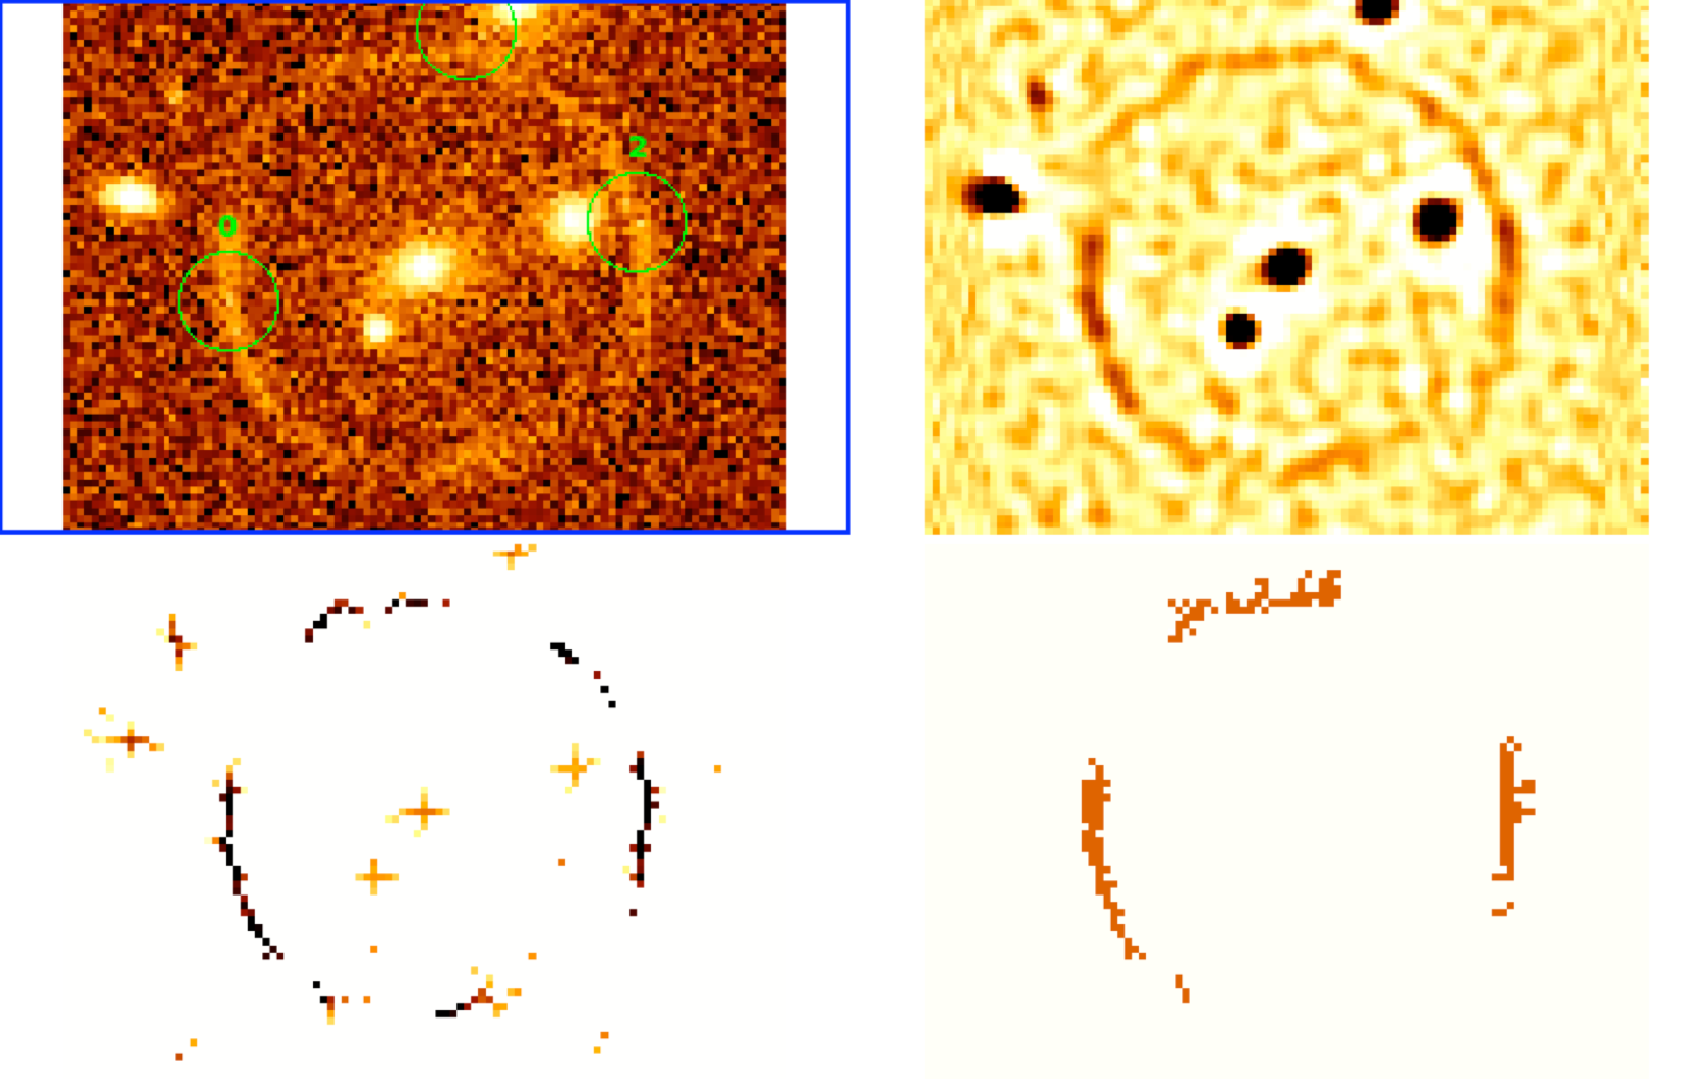
\includegraphics[width=\columnwidth]{Cabanac/arcmethod.pdf}
 \caption{ (GAHEC IRAP) From top-left to botton right, 1) a simulated arc extracted from SL challenge in which an tunned Arcfinder selects 3 candidates (green circles), 2) the smoothed image on which pixelwise elongation is computed, 3) the resulting elongated pixels after thresholding, 4) the set of pixels selected for the computation of arc candidate properties. }
 \label{fig:Cabanac}
\end{figure}

Arcfinder \citep{2006astro.ph..6757A,2007A&A...461..813C,2012ApJ...749...38M} is a fast linear method that computes a pixelwise elongation parameter (ratio of first-order moments in a n-pix window oriented in proper reference frame) for all pixels of mexican-hat-smoothed FITS images. Arcfinder then extract contiguous pixels above a given background and computes the candidate arcs length, width, area, radius of curvature and peak surface brightness. A final thresholding is set to maximize purity over completeness on a few typical arcs of the dataset.
For the current SL challenge, arcfinder was tunned to detect long and narrow arcs, and was optimized on a subset of 1000 simulated images with a grid covering a range of elongation windows and arc areas.  A python wrapper allows users to change parameters in a flexible way and run the arcfinder C code as a linux line command. Arcfinder took a couple of hours to run on the entire dataset with some overheads due to the dataset format. The code is publicly available at https://github.com/rcabanac/arcfinder.

\red{Reference to figure \ref{fig:Cabanac}?}

\subsection{AstrOmatic (Emmanuel Bertin)}

The lens detector is based on a convolutional neural network (CNN), trained with the provided training datasets. The CNN is implemented in Python, using the TensorFlow framework\footnote{http://www.tensorflow.org/}. Both ground multichannel and space monochannel image classifiers have the exact same CNN architecture.

The network itself consists of three convolutional layers ($11\times 11\times 32$, $5\times 5 \times 64$ and $3\times 3\times 64$), followed by two fully-connected layers ($256$ and $64$ neurons) and an output softmax layer. The first five layers use the ELU (Exponential Linear Unit) activation function \citep{2015arXiv151107289C}, which in our tests led to significantly faster convergence compared to ReLU and even SoftPlus activation. Dropout regularization \citep{2012arXiv1207.0580H,JMLR:v15:srivastava14a} is applied to both convolutional and fully connected layers, with ``keep'' probabilities $p=2/3$ and $p=1/2$, respectively.

Prior to entering the first convolutional layer, input image data are rescaled and dynamic-range compressed with function $f(x) =
\mathrm{arcsinh} (10^{11} x)$, and bad pixels are simply set to 0.
Data augmentation is performed in the form of random up-down and left-right image flipping, plus $k\pi/2$ rotations, where $k$ is a random integer in the $[0,3]$ range. Additionally, a small rotation with random angle $\theta$ is applied, involving bicubic image resampling. $\theta$ follows a Gaussian distribution with mean $\mu=0$ and standard deviation $\sigma_{\theta}=5^{\circ}$. No attempt was made to generate and randomize bad pixel masks in the data augmentation process.

The CNN weights are initialized to random values using a truncated Gaussian distribution with mean $\mu=0$ and standard deviation $\sigma=5.10^{-2}$. The network is trained on a Titan-X ``Pascal'' nVidia GPU using the Adam gradient-based optimizer \citep{2014arXiv1412.6980K} during 800 epochs, with an initial learning rate $\eta(t=0)=10^{-3}$ and a learning rate decay $\eta(t+1)/\eta(t)=0.99$, where $t$ is the epoch. Because of a lack of time, tests were limited to assessing the basic classification performance on a subset of the of 1,000 images/datacubes, using the 19,000 others for training.

\subsection{YattaLens Lite (Alessandro Sonnenfeld)}
YattaLensLite is a simpler version of the algorithm YattaLens \citep{Sonnenfeld17}, modified to meet the time constraints of the challenge.
YattaLensLite subtracts a model surface brightness profile describing the lens galaxy from the $g$-band image, then runs SExtractor to detect tangentially elongated or ring-shaped objects, which are interpreted as lensed images.
In the ground-based challenge, the model lens surface brightness profile is obtained by taking a rescaled version of the $i$-band image.
The difference in color between lens and source usually allows the lensed images to still be detectable after the lens subtraction process.
However in order to avoid subtracting off the lensed images in systems with similar colors between lens source, we radially truncate the model lens surface brightness.
at the smallest radius between the position where the surface brightness is comparable to the sky background level or the position of a positive radial gradient in surface brightness, if detected.

In the space-based challenge it is not possible to separate lens and source based on color, because only data in one band is provided. The lens light model then is produced by taking a centrally-inverted image and then using the same truncation prescription used with ground-based data. The central inversion step is taken to reduce the chances of subtracting flux from lensed images, which are in general not centrally symmetric as opposed to typical lens galaxies.

In the full version of YattaLens, a lens modeling step is performed to improve the purity of the sample. However, such a procedure is too time consuming and was not performed in this challenge.

\section{results}

\subsection{figures of merit}

In deriving a good figure of merit for evaluating lens finding algorithms one needs to take into account the particular nature of this problem.
The traditional method for evaluating a classification algorithm is with the receiver operating characteristic curve, or {\bf ROC} curve.  This a plot of the true positive rate (TPR) and the false positive rate (FPR).  In this case these are defined as
\begin{align}
{\rm TPR} &= \frac{\textrm{ number of true lenses classified as lenses}}{\textrm{ total number of true lenses}} \\
{\rm FPR} &= \frac{\textrm{number of non-lenses classified as lenses}}{\textrm{ total number of non-lenses}}
\end{align}
The classifier generally gives a probability of a case being a lens, $p$ in which case a threshold is set and everything with $p$ greater is classified as a lens and everything smaller classified as not a lens.  The TPR and FPR are then plotted as a curve parametrised by this threshold.  At $p=1$ all of the cases are classified as non-lenses and so TPR=FPR=1 and at $p=0$ all of the cases are classified as lenses so TPR=FPR=0.  These points are always added to the ROC curve.  If the classifier made random guesses then the ratio of lenses to non-lenses would be the same as the ratio of the number of cases classified as lens to the number of cases classified as non-lenses and so TPR=FPR.  The better a classifier is the smaller the FPR and the larger the TPR so the further away from this diagonal line it will be.  When a classifier provides only a binary classification or a discrete ranking the ROC connects the endpoints to the discrete points found be using each rank as a threshold.

A common figure of merit for a classifier is the area under the ROC ({\bf AUROC}).  This evaluates the overall ability of a classifier to distinguish between cases.  This was the criterion on which the challenge participants were told to optimize.  However, in the case of gravitational lensing this is not the only thing, and not the most important thing, to consider.  Gravitational lenses are rare events, but to improve the discrimination and training of the classifies the fraction lenses in the boosted to something around half.  In these circumstances it is important to consider the absolute number of cases that will be missclassified when the fraction of true cases is closer to what is expected in the data.

If the rates of false positives and false negatives remain the same in real data  the contamination of the sample will be
\begin{align}
\frac{\rm FP}{\rm TP} \simeq \frac{\rm FPR}{\rm TPR} \left(\frac{\textrm{number of non-lenses in sample}}{\textrm{number of lenses is sample}} \right)
\end{align}
Since only about one in a thousand objects will be lenses (perhaps somewhat more depending on pre-selection) the contamination will be high unless the FPR is much less than the TPR.  For this reason we consider some additional figures of merit.

The {\bf TPR0} will be defined as the highest TPR reached, as a function of $p$ threshold, before a single false positive occurs in the test set of 100,000 images.  This is the point were the ROC meets the FPR = 0 axis.  This quantity highly penalizes classifiers with discrete ranking which often get TPR0 = 0 because their highest classification level is not conservative enough to eliminate all false positives.  We also define {\bf TPR10} which is the TPR at the point were less than ten false positives are made.  If the TP 
rate is boosted from the FPR by a factor of 1,000 in a realistic data set with would correspond to about a 10\% contamination.

In addition to these considerations, the performance of a classifier is a function of many characteristics of the lens system.  It might be that one classifier is good at finding systems with large Einstein radii and incomplete arcs, but not as good at finding small complete Einstein rings that are blended with the light of the lens galaxy.  Also lens may have a source that is too faint to be detected by any algorithm or is too far from the lens to be very distorted, but will be classified as a lens in the test data set.   We want to include these objects because we want to test the limits of the classifiers.  As we will see, if you restrict your objectives to detecting only lensed images with surface brightness above threshold, for example, the "best" algorithm might change and the TPR will change.  For this reason we plot the AUROC, TPR0 and TPR10 as a function of several variables for all the entries.  This is done by removing all the lenses that do not exceed the threshold and then recalculating the these quantities, the number of non-lenses remains the same.

***
\subsection{plots}


\section{Conclusions \& discussion}

It is clear that the robustness of lens finders against falsely classifying unusual galaxies as lenses was not adequately tested in this challenge.  Some of the methods which appear overly conservative in this test might be better at avoiding false positives in real data.  This can be seen as a form of over fitting to the test set.
In future challenges we wish to concentrate on this aspect of the problem.

Human inspection was the only method to find the jackpot lens

\section*{Acknowledgements}

EB thanks Raphael Gavazzi for proposing him to participate to the challenge.
AS was supported by World Premier International Research Center Initiative (WPI Initiative), MEXT, Japan.
RBM's research was partly part of project GLENCO, funded under the European Seventh Framework Programme, Ideas, Grant Agreement n. 259349.

%%%%%%%%%%%%%%%%%%%%%%%%%%%%%%%%%%%%%%%%%%%%%%%%%%
%%%%%%%%%%%%%%%%%%%% REFERENCES %%%%%%%%%%%%%%%%%%

\bibliographystyle{mn2e}
\bibliography{references}

%%%%%%%%%%%%%%%%%%%%%%%%%%%%%%%%%%%%%%%%%%%%%%%%%%
%%%%%%%%%%%%%%%%% APPENDICES %%%%%%%%%%%%%%%%%%%%%

\appendix

\label{lastpage}
\end{document}
